\subsection{Theoretische Physik 1 - Mechanik und Mathem. Methoden}
\label{theo1}
Die Theoretische Physik 1 (\gls{Theo}) beschäftigt sich mit der Newton'schen Mechanik und nützlichem mathematischen Werkzeug.

Hier werdet ihr im ersten Semester einige Zusammenhänge und Techniken einfach „vorgesetzt“ bekommen ohne sie völlig zu verstehen. Der genaue Grund, warum ihr das, was ihr da tut, eigentlich dürft, wird im Normalfall erst in einer der späteren Mathevorlesungen klar, daran solltet ihr aber nicht verzweifeln. Dieses Vorgehen ist in der Physik nicht ungewöhnlich, was einer der Angriffspunkte von Witzen der Mathematikerinnen über Physikerinnen ist\dots

Ihr erhaltet hier aber nicht nur die mathematischen Techniken, die ihr in Eurem Studium brauchen werdet (und von denen ihr in vielen Fällen noch nie was gehört habt), sondern Euch wird auch eine theoretische Beschreibung der Mechanik vorgestellt. Diese unterscheidet sich im ersten Semester, bis auf einige seltsame Symbole und unglaubliche Umständlichkeit noch nicht sehr von der in der Experimentalphysik 1 \gls{Ex}, ab dem zweiten Semester tun sich zwischen den Sichtweisen jedoch Abgründe auf und ihr werdet verstehen, warum auf diese Umständlichkeit bestanden wurde.

Der Anspruch dieser Vorlesung an Verständnis und Wissen ist deutlich größer als in der Ex 1, womit ihr auch einen erheblich höheren Aufwand für die Bewältigung der Arbeitszettel einplanen könnt, je nach eigenem Interesse, Wissen und Perfektionismus sind zehn Stunden durchaus eine realistische Einschätzung für einen Zettel. Die Übungsgruppenleiterinnen sind hier vor allem ältere Studierende, was den Vorteil hat, dass diese sich noch an ihre eigenen Probleme in ihrer Theo 1 erinnern können und Euch das ganze verständlicher erklären können als die Theo-Prof es kann.

\vfill
\begin{figure}[hbt]
	\centering{
    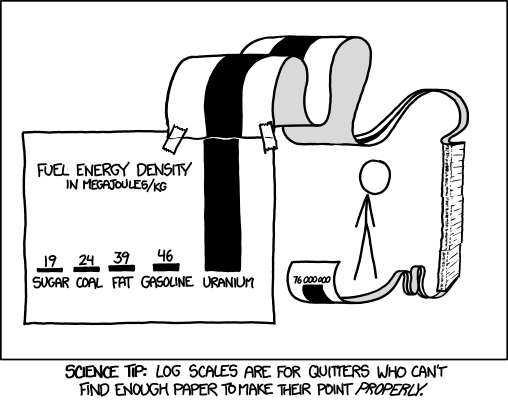
\includegraphics[width=\textwidth]{bilder/log_scale.png}
}
\end{figure}